\subsection{Diseño experimental}
\begin{itemize}[leftmargin=*,itemsep=1pt]
\item \textbf{Árbol:} MDFD con máscaras ideales en FFT, $F_s=12$~kHz y $L=6$ (hojas de 93{,}75~Hz). Es la misma implementación del curso.
\item \textbf{Criterio de diagnóstico, idéntico para todos los métodos:} en el SES de la banda elegida, la relación armónica/fondo en $f_d\pm2\%$ debe ser $\ge 6$~dB. El fondo es la mediana del SES en $f_d\pm0{,}3f_d$, sin contar el pico.
\item \textbf{Simulación:} falla de pista externa, $f_d=107{,}3$~Hz, con 1\% de deslizamiento aleatorio. Cada impacto excita una resonancia de $f_n=3{,}5$~kHz y $\zeta=0{,}04$. Hay 10~s de señal más ruido gaussiano (el SNR se mide sobre la potencia total de la falla). Escenarios:
A)~base;
B)~$+$~impactos aleatorios (Poisson, 3/s) en otra resonancia de 1{,}2~kHz;
C)~$+$~holgura: impactos a $f_r$ en 5{,}2~kHz;
D)~$+$~EMI (40 armónicos de 60~Hz) y tonos de giro/engrane;
E)~resonancia en 3~kHz, que cae sobre una frontera diádica en \emph{todos} los niveles.
Se hicieron 8 réplicas por celda.
\item \textbf{CWRU:} los 105 registros con falla a 12~kHz (60 DE y 45 FE). $f_d$ es BPFI, BPFO o $2\,$BSF, igual que en la clase para el registro 282. Para medir falsas alarmas de forma justa, cada registro también se evalúa en dos \emph{frecuencias señuelo} ($2{,}68f_r$ y $3{,}79f_r$ en DE; $2{,}47f_r$ y $5{,}47f_r$ en FE). Estas frecuencias están elegidas lejos de toda línea cinemática conocida (armónicos de $f_r$, BPFI, BPFO, BSF, $2\,$BSF, FTF y bandas laterales). Un método útil debe detectar en $f_d$ y \emph{no} en los señuelos. Se reporta $J=\text{TPR}-\text{FPR}$ (índice de Youden).
\end{itemize}

\subsection{Mapas: qué ve cada métrica}
\begin{figure}[!htb]
\centering
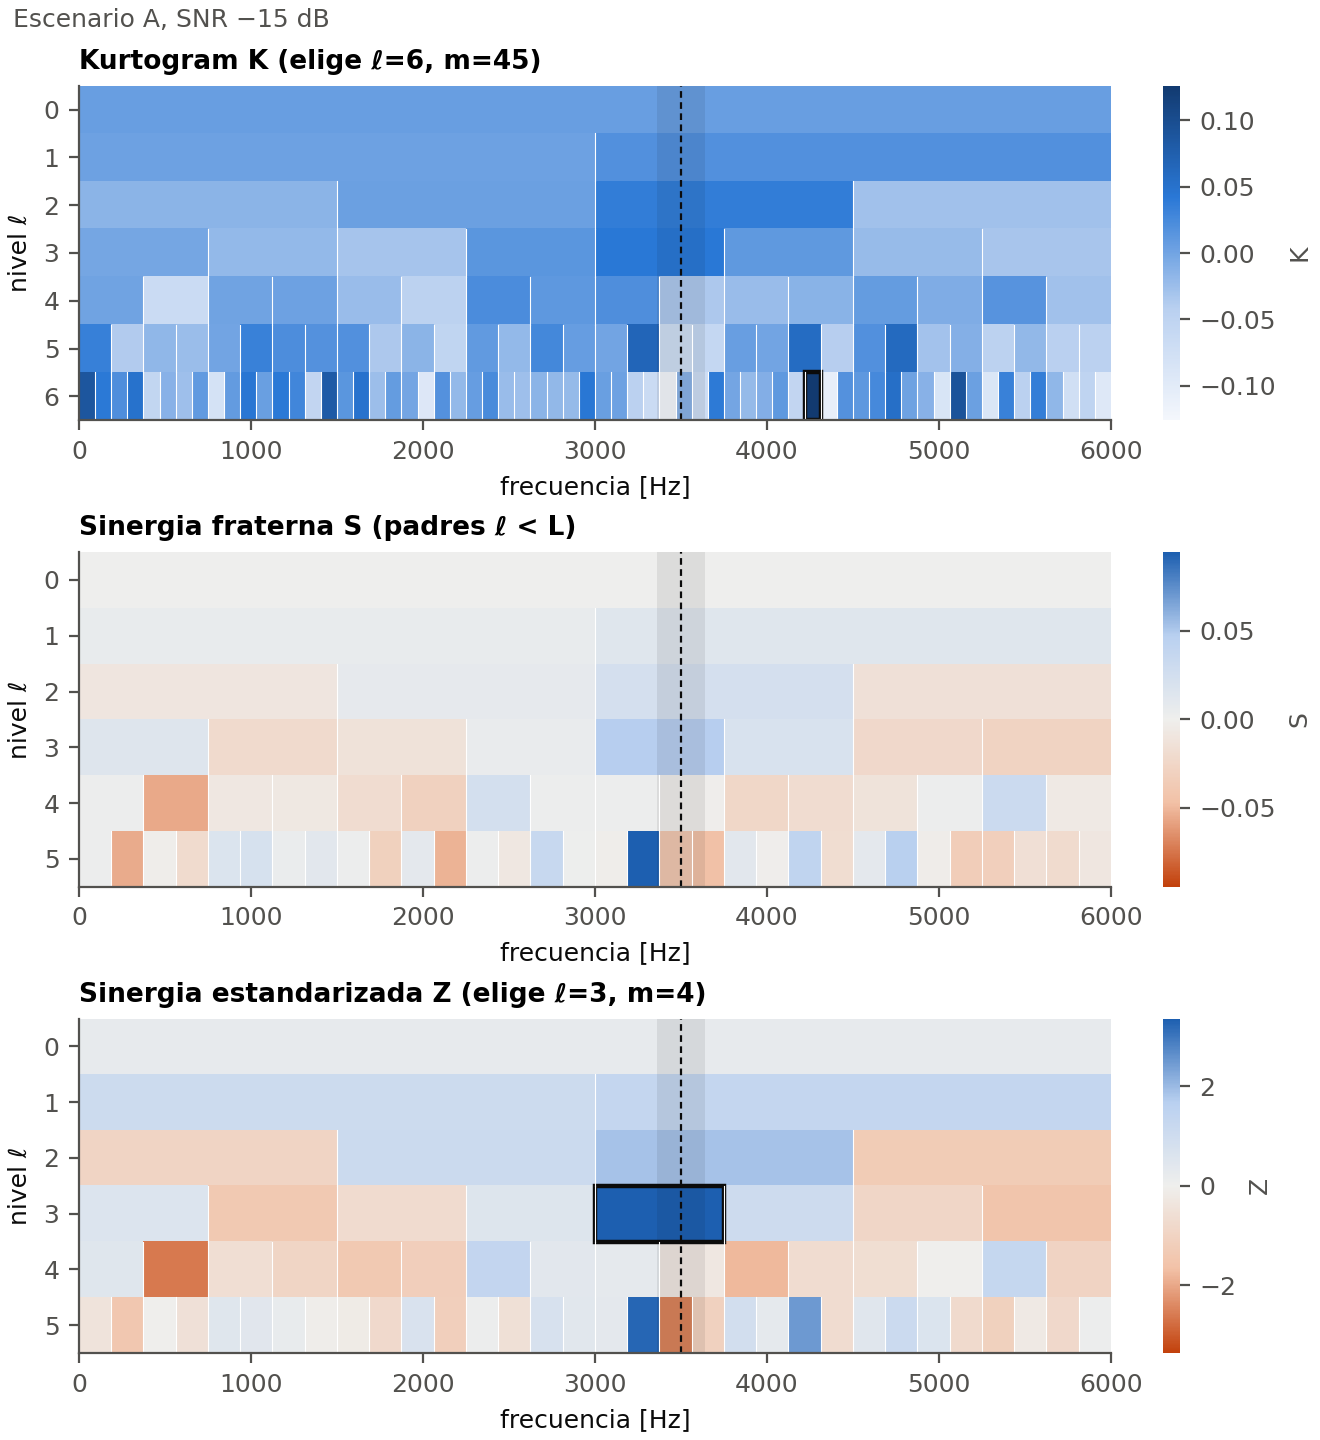
\includegraphics[width=0.84\textwidth]{../fig/mapas_base.png}
\caption{Escenario A, SNR $-15$~dB. El kurtogram elige un nodo del nivel 6 de 94~Hz de ancho, \emph{más angosto que $f_d$}, así que el diagnóstico es imposible. Es el sesgo de profundidad predicho por el Corolario~\ref{cor:sesgo} y la Proposición~\ref{prop:var}. El sinergograma $Z$ elige 3000--3750~Hz, que contiene la resonancia (franja gris), y el SES de esa banda muestra $f_d$ con 8{,}6~dB.}
\label{fig:mapasA}
\end{figure}

\begin{figure}[!htb]
\centering
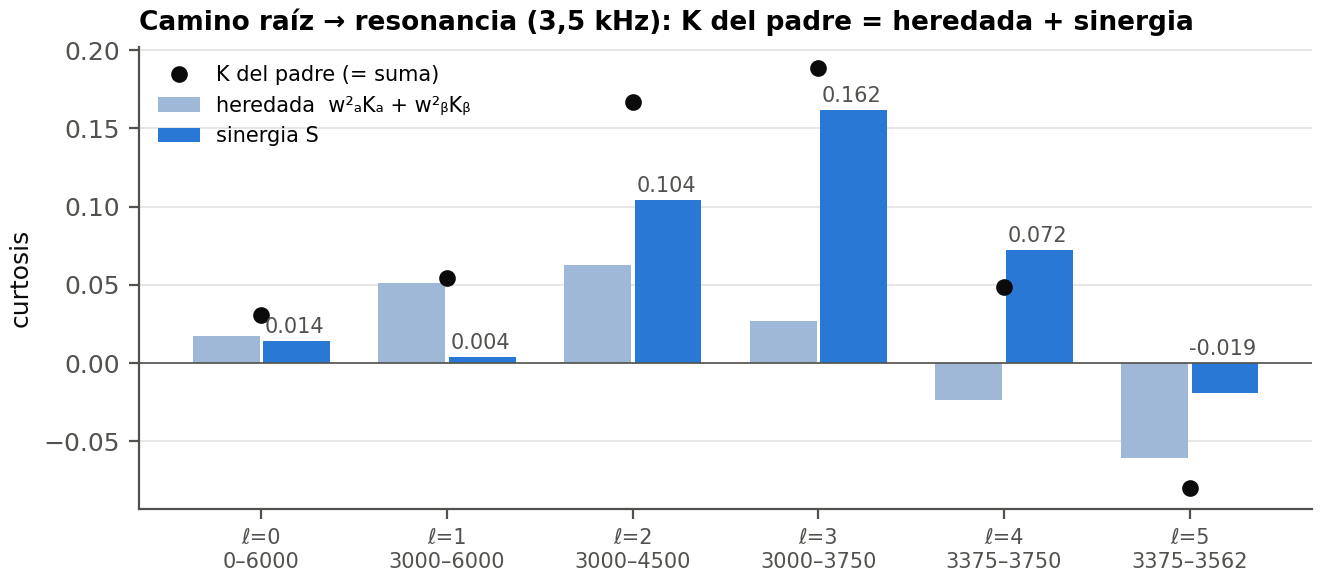
\includegraphics[width=0.8\textwidth]{../fig/herencia.png}
\caption{Identidad \eqref{eq:herencia} a lo largo del camino raíz$\to$resonancia (SNR $-12$~dB). En $\ell=1$ (3--6~kHz, un hijo con la resonancia y otro con ruido) la curtosis del padre es casi toda heredada. En $\ell=2$ y $3$ domina la sinergia: la resonancia ocupa a ambos hijos. En $\ell=4$ la parte heredada ya es negativa y sólo la sinergia sostiene $K$. En $\ell=5$ los hijos (94~Hz) son más angostos que $f_d$ y no pueden contener la modulación: ambas partes son negativas.}
\label{fig:herencia}
\end{figure}

\begin{figure}[!htb]
\centering
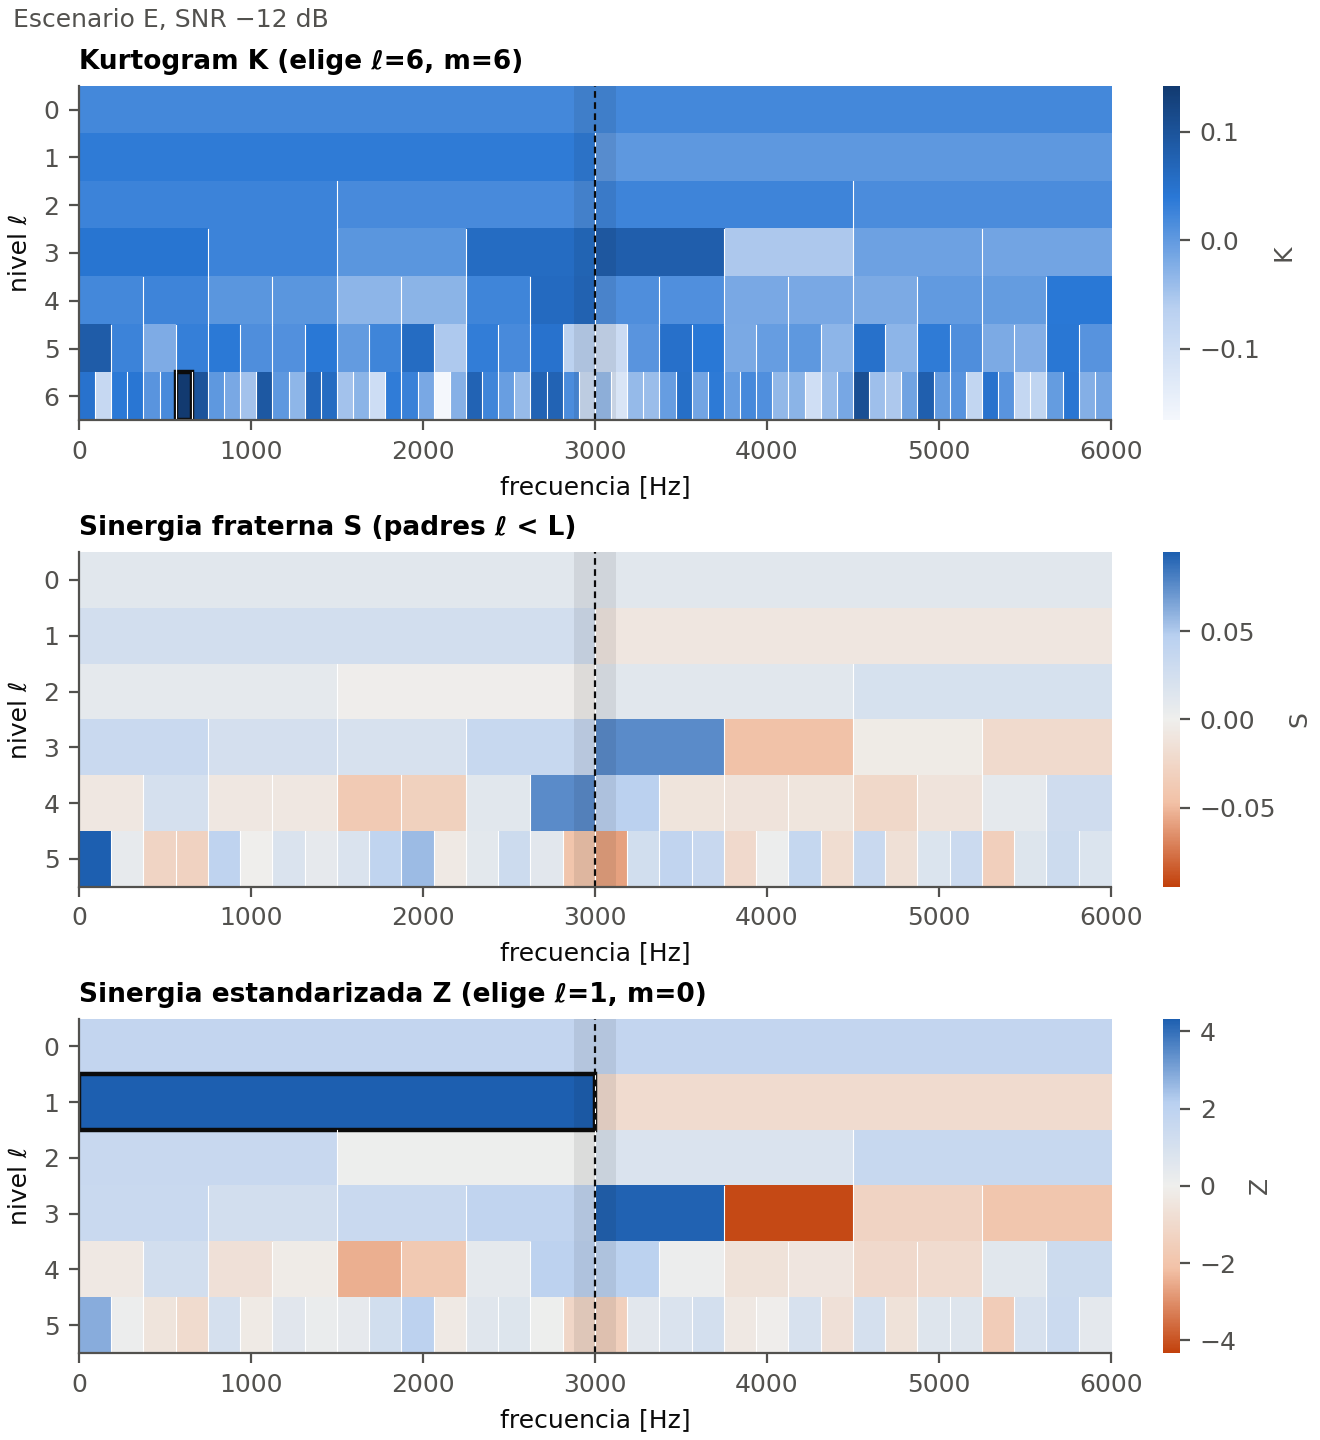
\includegraphics[width=0.84\textwidth]{../fig/mapas_frontera.png}
\caption{Escenario E (resonancia en 3~kHz, sobre una frontera diádica), SNR $-12$~dB. El kurtogram vuelve a caer en un nodo de 94~Hz lejos de la resonancia (562--656~Hz). $Z$ elige 0--3000~Hz, que contiene la mitad inferior de la resonancia, y también marca 3000--3750~Hz, la mitad superior. La sinergia sigue a la resonancia a ambos lados de la frontera, aunque ningún nodo diádico la contenga entera. Esto motiva la idea 6 (sinergia entre primos).}
\label{fig:mapasE}
\end{figure}

\subsection{Monte Carlo en simulación}
\begin{figure}[!htb]
\centering
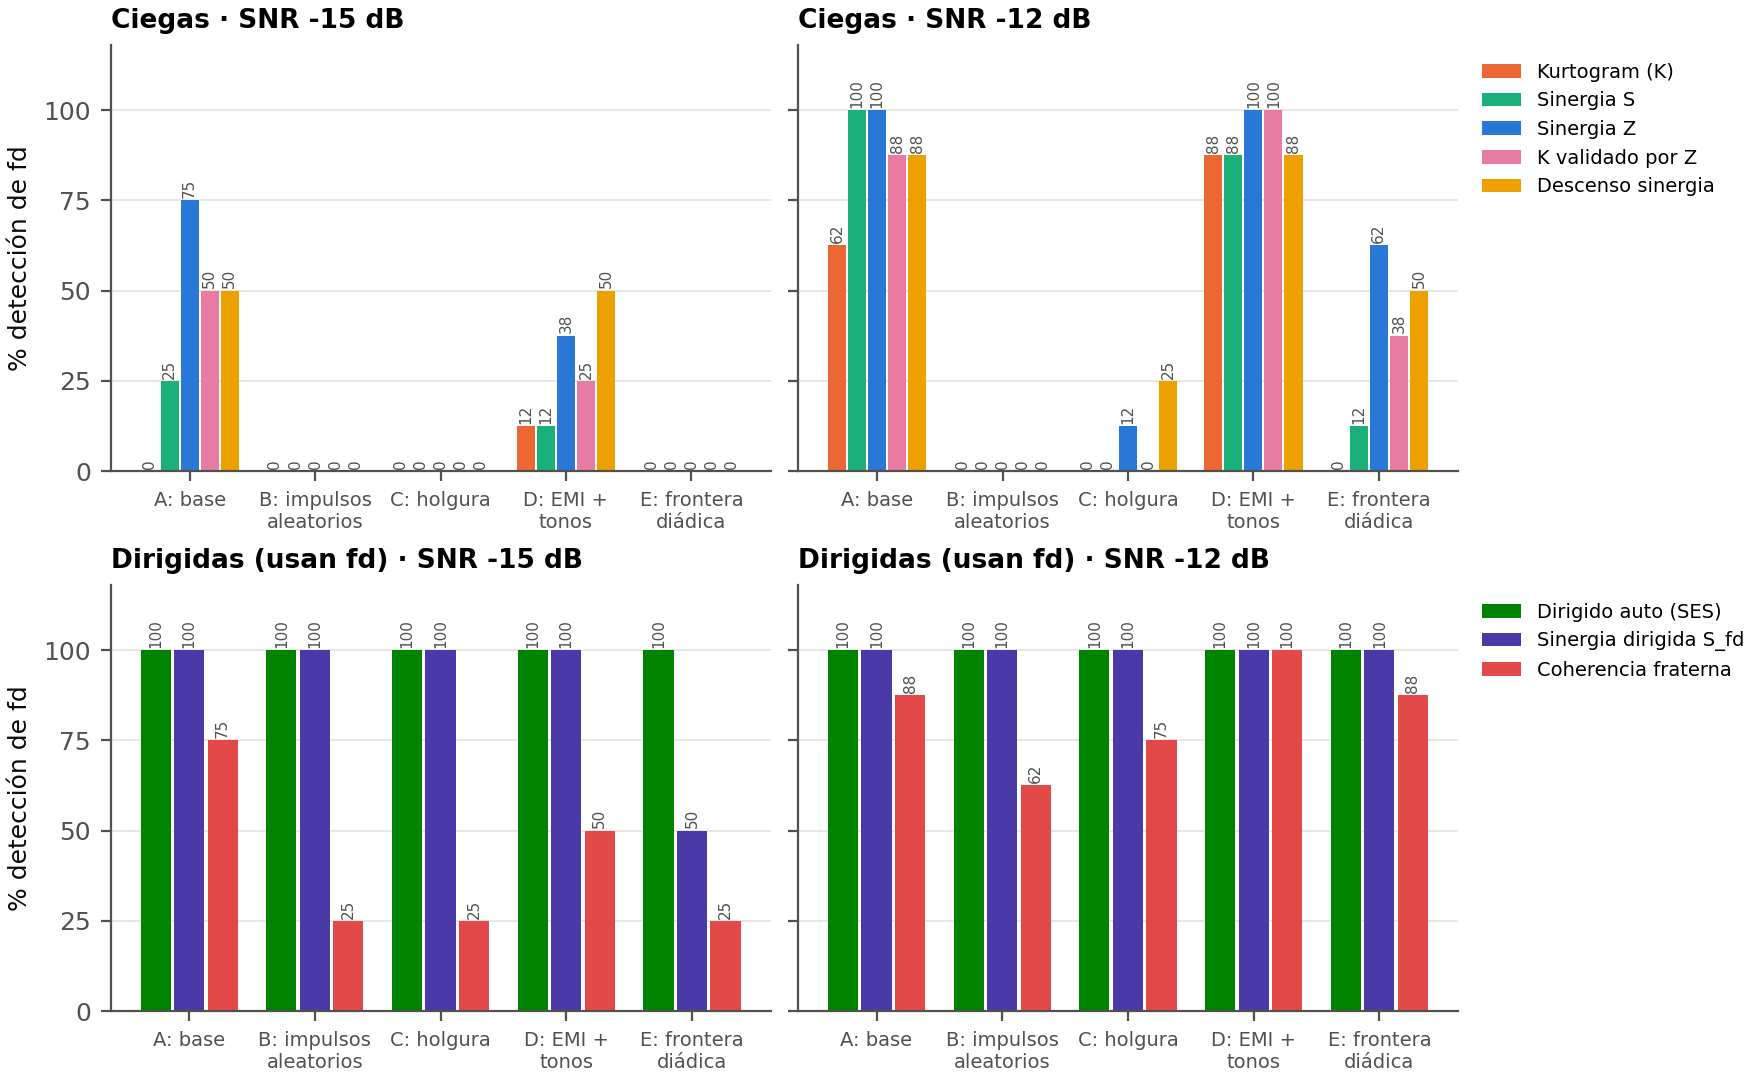
\includegraphics[width=\textwidth]{../fig/montecarlo.png}
\caption{Porcentaje de réplicas en que la banda elegida permite ver $f_d$ (8 réplicas por barra). A $-18$~dB ningún método ciego detecta (no se muestra).}
\label{fig:mc}
\end{figure}

\begin{table}[!htb]
\centering\small
\begin{tabular}{@{}lccccc|ccccc@{}}
\toprule
& \multicolumn{5}{c|}{SNR $-15$ dB} & \multicolumn{5}{c}{SNR $-12$ dB}\\
Método (ciego) & A & B & C & D & E & A & B & C & D & E\\
\midrule
Kurtogram $K$ (clase) & 0 & 0 & 0 & 12 & 0 & 62 & 0 & 0 & 88 & 0\\
Sinergia $S$ & 25 & 0 & 0 & 12 & 0 & \textbf{100} & 0 & 0 & 88 & 12\\
\textbf{Sinergia $Z$} & \textbf{75} & 0 & 0 & 38 & 0 & \textbf{100} & 0 & 12 & \textbf{100} & \textbf{62}\\
Descenso por sinergia & 50 & 0 & 0 & \textbf{50} & 0 & 88 & 0 & \textbf{25} & 88 & 50\\
\bottomrule
\end{tabular}
\caption{Detección (\%) de los métodos ciegos en simulación.}
\label{tab:mc}
\end{table}

\noindent\textbf{Lectura.}
(1) Con ruido gaussiano, EMI y tonos (A, D) y con resonancia en frontera (E), la sinergia estandarizada supera claramente al kurtogram: 75 contra 0\% en A a $-15$~dB y 62 contra 0\% en E a $-12$~dB. Los tonos y la EMI no la engañan, como predice la tabla de interpretación física.
(2) Con impactos que \emph{no} vienen del rodamiento (B aleatorios, C holgura), todos los métodos ciegos fallan, incluida la sinergia. Es la limitación honesta de cualquier criterio de impulsividad y motiva la versión cíclica.
(3) Las métricas dirigidas (fila inferior de la Fig.~\ref{fig:mc}) detectan casi siempre desde $-15$~dB. La sinergia dirigida $S_{f_d}$ empata con el índice dirigido clásico salvo en E a $-15$~dB. La coherencia fraterna normalizada rinde menos. \emph{En simulación no se controló la falsa alarma de los métodos dirigidos}; eso se mide en CWRU.

\subsection{CWRU}
\begin{figure}[!htb]
\centering
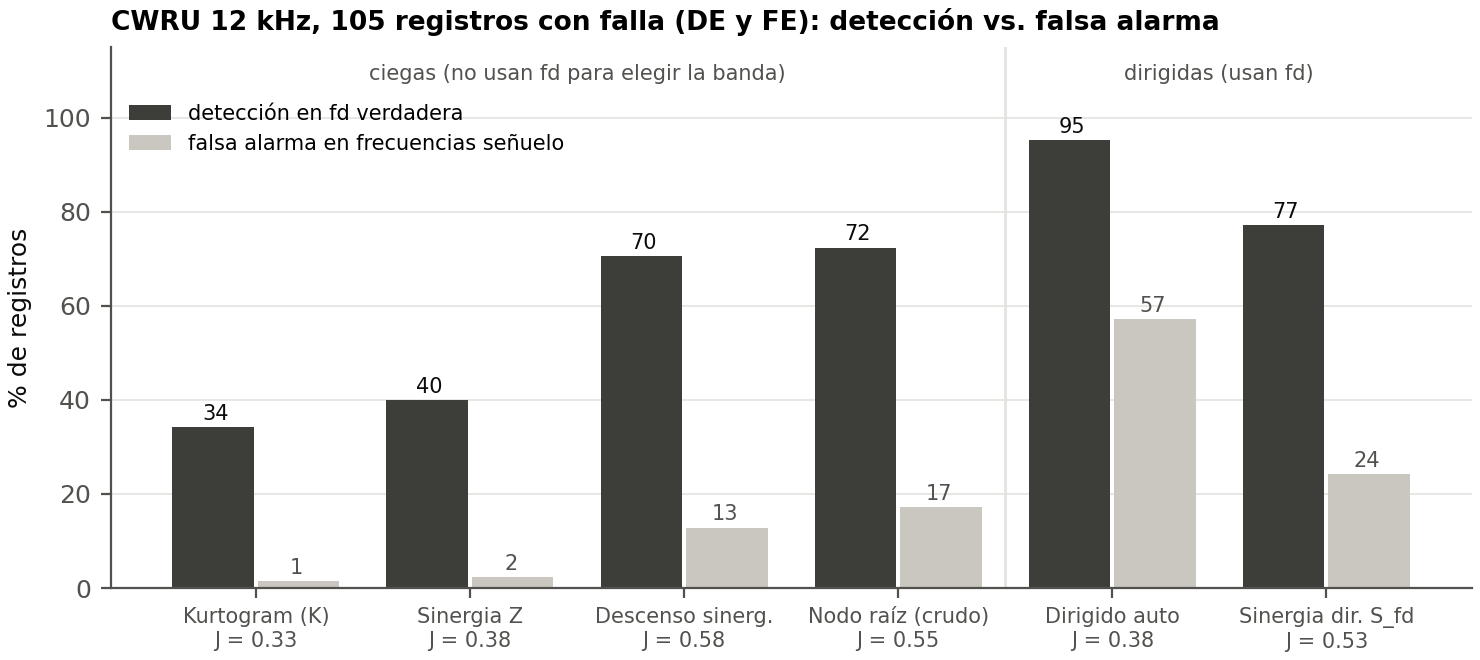
\includegraphics[width=0.95\textwidth]{../fig/cwru_resumen.png}
\caption{Detección en la $f_d$ verdadera frente a detección en frecuencias señuelo (falsa alarma) y $J=$TPR$-$FPR.}
\label{fig:cwru}
\end{figure}

\begin{table}[!htb]
\centering\footnotesize\setlength{\tabcolsep}{4pt}
\begin{tabular}{@{}lccc|ccc|cc|c@{}}
\toprule
& \multicolumn{3}{c|}{Categoría Smith--Randall} & \multicolumn{3}{c|}{Tipo de falla} & \multicolumn{2}{c|}{Sensor} & FA \\
Método & Y (70) & P (17) & N (18) & IR (28) & OR (49) & B (28) & DE (60) & FE (45) & señuelos\\
\midrule
Kurtogram $K$ & 37 & 35 & 22 & 39 & 47 & 7 & 3 & 76 & 1\\
Sinergia $Z$ & 51 & 29 & 6 & 50 & 51 & 11 & 18 & 69 & 2\\
Descenso por sinergia & 93 & 35 & 17 & 89 & 84 & 29 & 72 & 69 & 13\\
Nodo raíz (SES crudo) & 94 & 35 & 22 & 93 & 84 & 32 & 77 & 67 & 17\\
\midrule
Dirigido auto (SES) & 99 & 88 & 89 & 93 & 98 & 93 & 93 & 98 & 57\\
Sinergia dirigida $S_{f_d}$ & 96 & 47 & 33 & 93 & 94 & 32 & 78 & 76 & 24\\
\bottomrule
\end{tabular}
\caption{CWRU 12~kHz: \% de registros con $f_d$ visible, por grupo, y falsa alarma (FA, \%) en señuelos.}
\label{tab:cwru}
\end{table}

\noindent\textbf{Lectura honesta de CWRU.}
\begin{enumerate}[leftmargin=*,itemsep=2pt]
\item \textbf{$Z$ contra el kurtogram:} 40 contra 34\% de detección con la misma falsa alarma (2 y 1\%). En la comparación pareada, $Z$ gana en 10 registros y pierde en 4. La mejora es real pero moderada.
\item \textbf{Ambos pierden contra la envolvente de la señal cruda (72\%).} La causa se ve en la Fig.~\ref{fig:cwru105}: muchos registros DE contienen ráfagas impulsivas \emph{ajenas al rodamiento}, concentradas en bandas angostas (en el registro 105, $K\approx200$ en 5{,}9--6~kHz, junto a Nyquist). El kurtogram las elige y sólo detecta el 3\% de los registros DE. $Z$ también cae en ellas, porque un impulso aislado co-modula a los hermanos (escenario B). Esto es coherente con lo que Smith \& Randall (2015) describen en CWRU: EMI con portadoras de alta frecuencia (armónicos de $\sim$4{,}2~kHz con bandas laterales a $f_r$), armónicos altos del giro atribuibles a holgura y pulsos aparentemente aleatorios en varios registros.
\item \textbf{El descenso por sinergia}, la regla que usa el árbol de forma explícita, detecta el 70\% (43 aciertos donde el kurtogram falla, contra 5 al revés) y tiene menos falsa alarma que la señal cruda (13 contra 17\%). En 65 de 105 registros se detiene en el nivel 1: en CWRU los impactos co-modulan media banda de Nyquist completa, así que la identidad dice ``no dividas más''.
\item \textbf{Métricas dirigidas:} el índice clásico (energía del SES en armónicas de $f_d$, del tipo ICS2/RCC) ``detecta'' el 95\%, pero también el 57\% de los señuelos. Al buscar entre 127 bandas la que tiene más energía en \emph{cualquier} frecuencia, casi siempre encuentra algo: es un problema de comparaciones múltiples. La \textbf{sinergia dirigida} detecta el 77\% con 24\% de falsa alarma y logra el mejor $J$ entre las dirigidas (0{,}53 contra 0{,}38). Es lo que predice la Proposición~\ref{prop:insesgo}: en el espectro cruzado entre hermanos el ruido no genera picos positivos.
\item El registro 282 de clases (Fig.~\ref{fig:cwru282}) es categoría N en Smith \& Randall para el sensor FE con los tres métodos. Ningún método ciego lo diagnostica, y la falta de diagnóstico es consistente con esa referencia.
\end{enumerate}

\begin{figure}[!htb]
\centering
\begin{minipage}[t]{0.495\textwidth}\centering
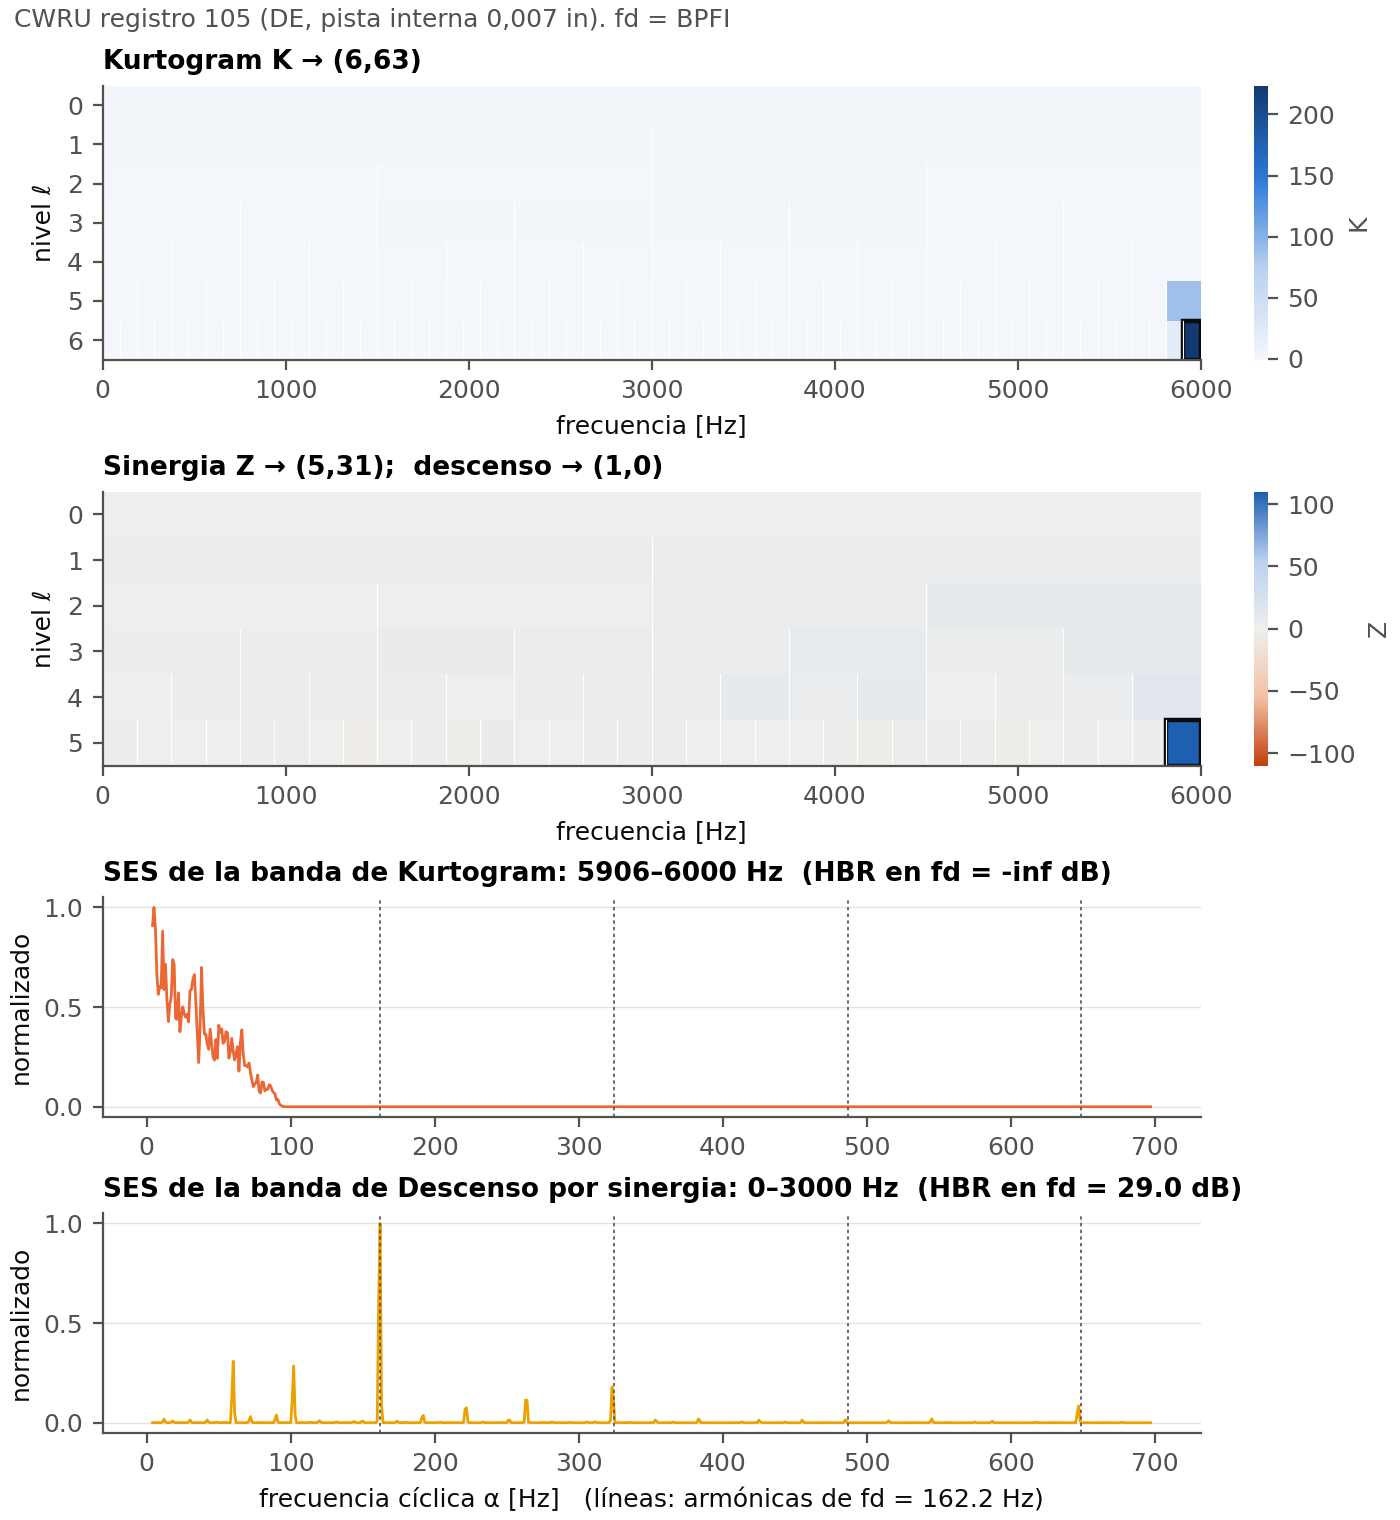
\includegraphics[width=\linewidth]{../fig/cwru_105.png}
\captionof{figure}{Registro 105 (DE, pista interna). El kurtogram elige 5906--6000~Hz por una ráfaga no relacionada con la falla. El descenso por sinergia se detiene en 0--3000~Hz y el SES muestra BPFI con 29~dB.}
\label{fig:cwru105}
\end{minipage}\hfill
\begin{minipage}[t]{0.495\textwidth}\centering
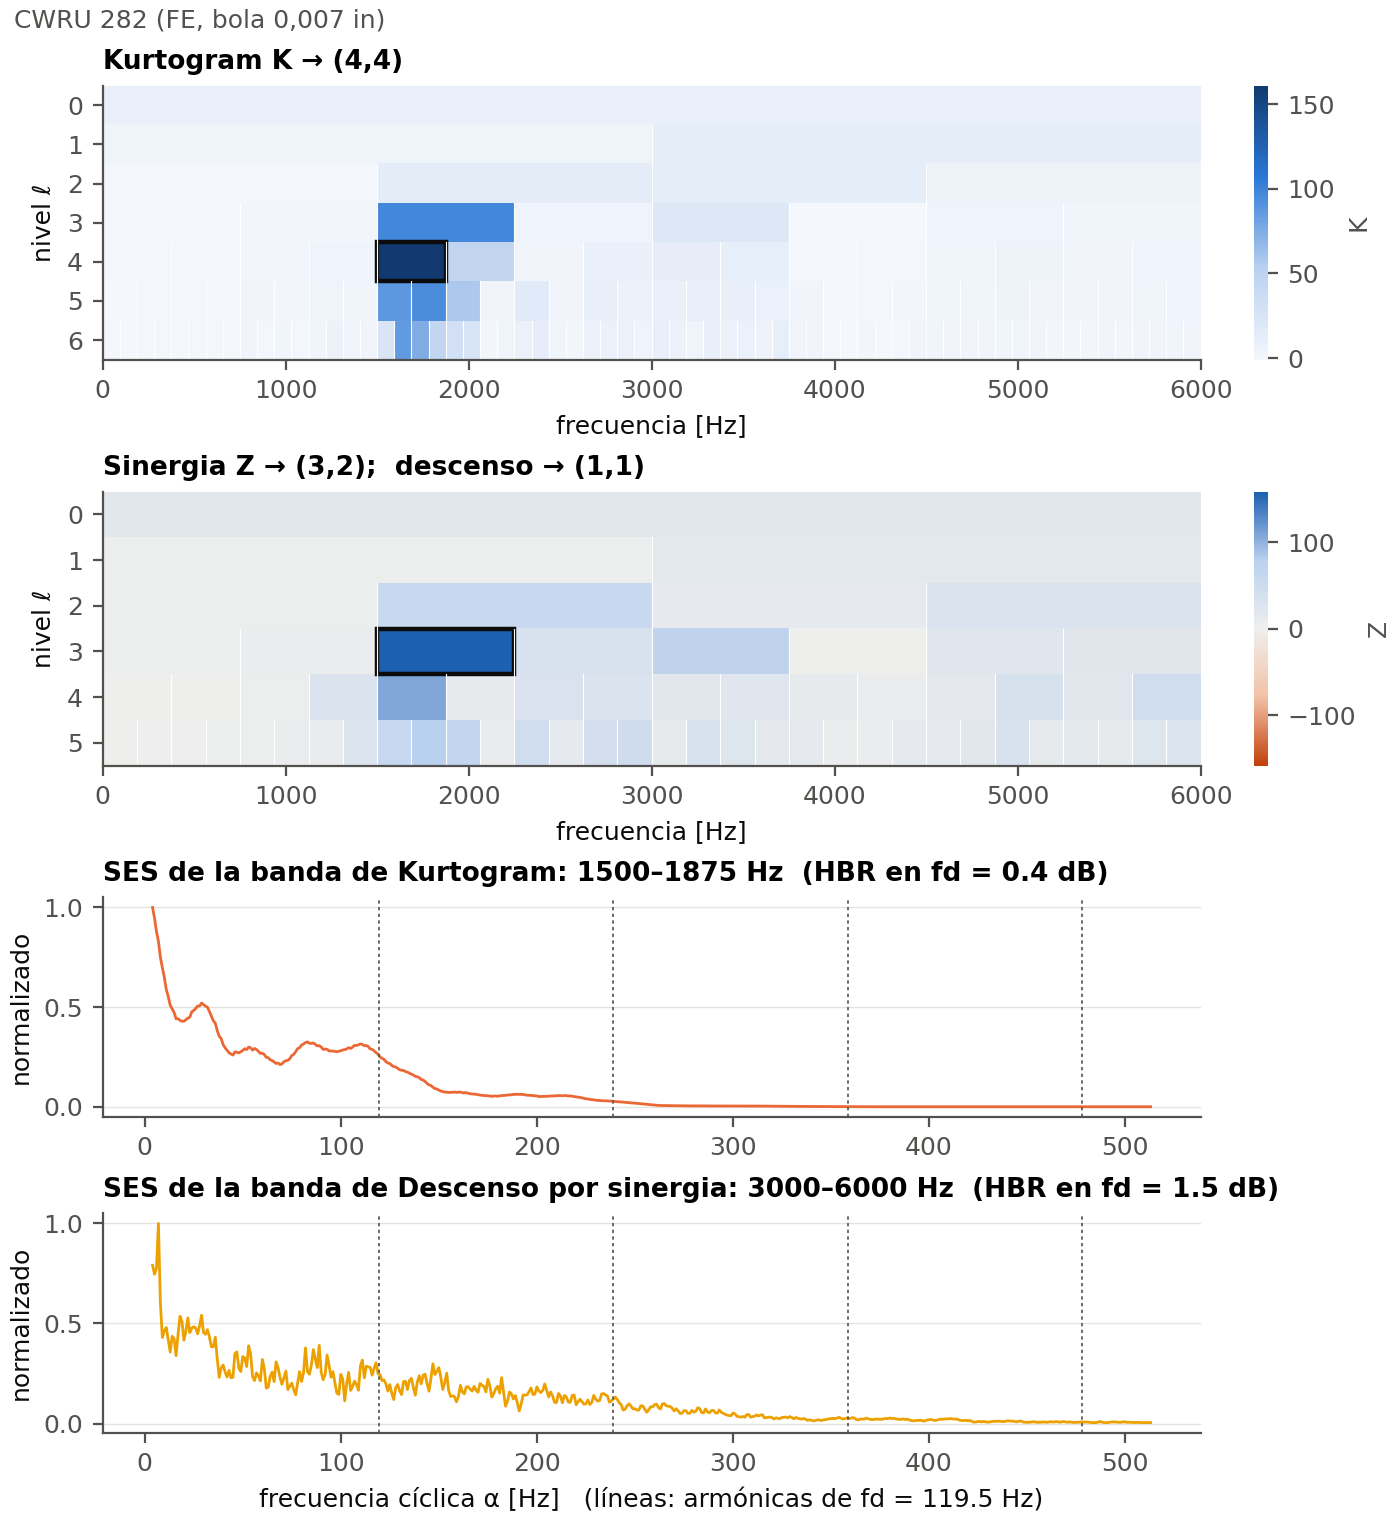
\includegraphics[width=\linewidth]{../fig/cwru_282.png}
\captionof{figure}{Registro 282 (ejemplo de clase, FE, bola 0{,}007 in). $2\,$BSF $=119{,}5$~Hz no aparece con ningún método ciego. Es un registro ``no diagnosticable'' según el benchmark de Smith \& Randall.}
\label{fig:cwru282}
\end{minipage}
\end{figure}

\subsection{Conclusiones}
\begin{enumerate}[leftmargin=*,itemsep=2pt]
\item El árbol MDFD admite una \textbf{identidad exacta} ($K_p=w_a^2K_a+w_b^2K_b+S_p$) que separa la curtosis de un nodo en lo heredado de sus hijos y lo que emerge de su interacción. Es el aporte central: convierte la estructura del árbol en información.
\item La identidad \textbf{explica} el principal defecto del kurtogram: sin sinergia la curtosis se diluye al subir por el árbol, y el ruido de estimación crece como $2^{\ell/2}$ al bajar. Por eso el $\arg\max$ resbala hacia hojas inútiles: a $-15$~dB el kurtogram detectó 0\% en 4 de los 5 escenarios.
\item La \textbf{sinergia estandarizada} $Z$ corrige ese sesgo en ruido gaussiano, EMI, tonos y resonancias en frontera diádica. En CWRU mejora al kurtogram de forma moderada.
\item Las dos variantes que usan el árbol de forma más explícita dieron los mejores compromisos detección/falsa alarma de sus familias en CWRU: el \textbf{descenso por sinergia} ($J=0{,}58$) y la \textbf{sinergia dirigida} ($J=0{,}53$).
\item Ninguna métrica de impulsividad ciega distingue impactos del rodamiento de impactos ajenos. La vía natural es la \textbf{sinergia cíclica ciega} (idea 10), que busca en $s_p(\alpha)$ un peine armónico sin conocer $f_d$.
\end{enumerate}
